\documentclass{article}

\renewcommand{\familydefault}{\sfdefault}  %serifenlose Schrift
\usepackage{helvet} % Schrift: Helvetica


\usepackage{graphicx,graphics,tikz}
\usepackage{amsmath}
\usepackage{amsthm}
\usepackage{amsfonts}
\usepackage{amssymb}
\usepackage{marvosym} % to be able to show male and female symbols with: \Female and \Male
\usepackage{gensymb}
\usepackage[graphics,tightpage,active]{preview}
\PreviewEnvironment{tikzpicture}
\newlength\imagewidth
\newlength\imagescale

\begin{document}

\pgfmathsetlength{\imagewidth}{10cm} % desired displayed width of image
\pgfmathsetlength{\imagescale}{\imagewidth/2000} % pixel width of image
% adjust scale of tikzpicture (and direction of y) such that pixel
% coordinates can be used for drawing overlays:
\usetikzlibrary{backgrounds}

\begin{tikzpicture}[x=\imagescale,y=-\imagescale]

\node [text centered] at (3.75cm,2.7cm) {\textbf{Zygote dispersal: \textless 10m}};
\node [text centered] at (1cm,2cm) {\textbf{Flotation vesicles}};
\node at (1.5cm,-1.5cm) {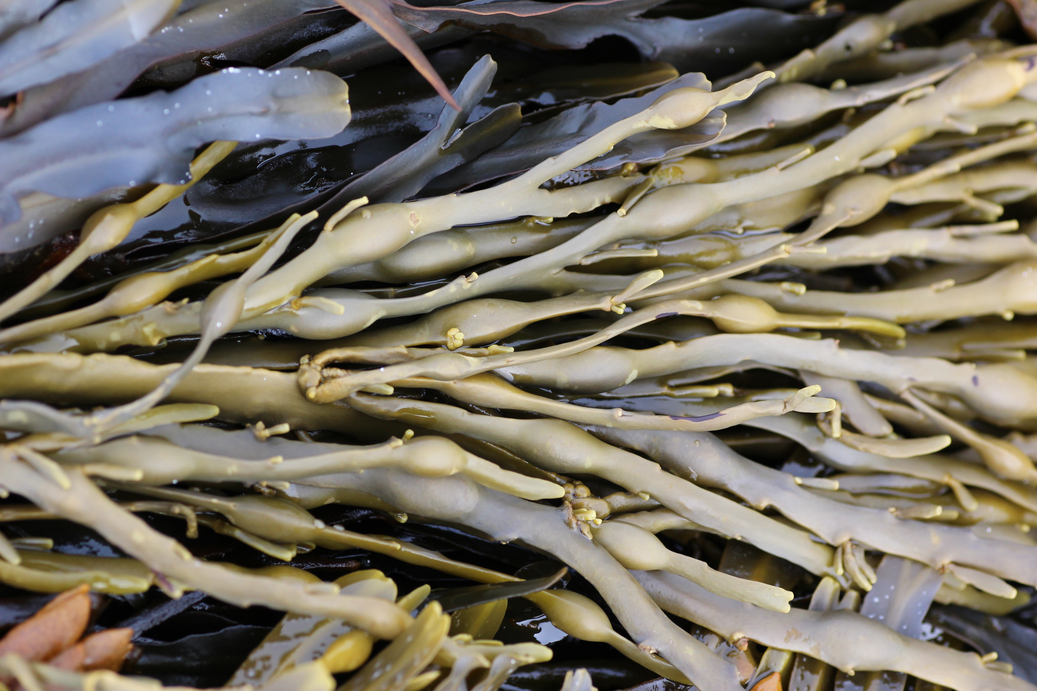
\includegraphics[width=3cm]{IMG_1503_r.png}};
\node at (0cm,0cm) {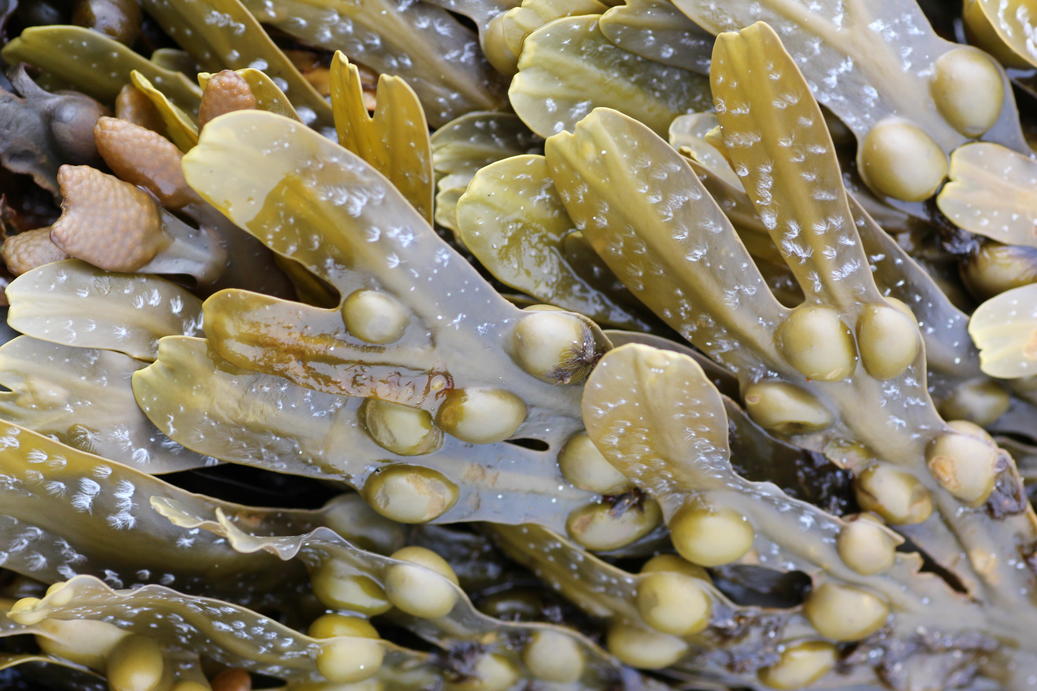
\includegraphics[width=3cm]{IMG_1498_r.png}};

\node [text width=3cm, text centered] at (0cm,1.3cm) {\scriptsize{\textit{Fucus} \textit{vesiculosus}}};
\node [text width=3cm, text centered] at (1.5cm,-3cm) {\scriptsize{\textit{Ascophyllum} \textit{nodosum}\\ \textbf{low invasive potential}}};


\node at (6.5cm,2cm) {\textbf{Shipping transport}};
\node at (6.5cm,0cm) {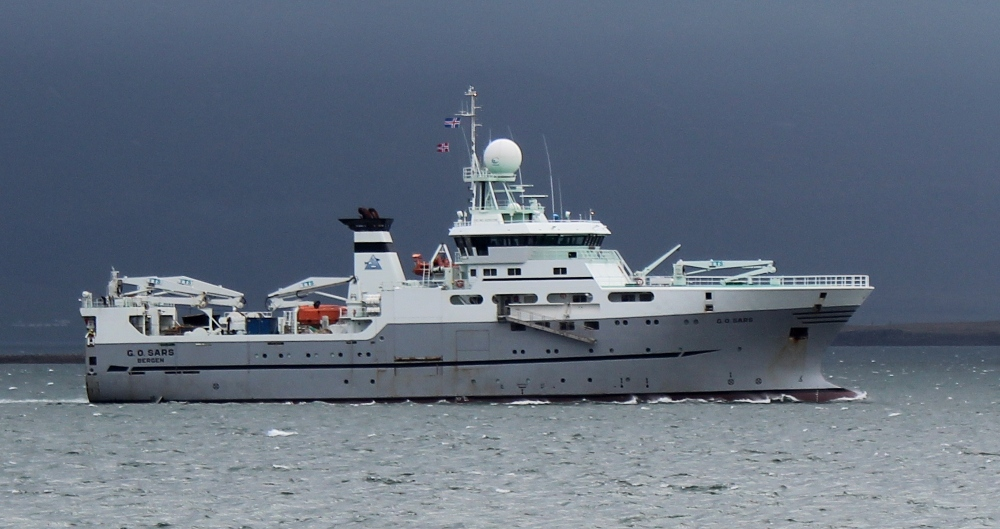
\includegraphics[width=5cm]{IMG_2987_r.png}};
\node at (8.3cm,-2cm) {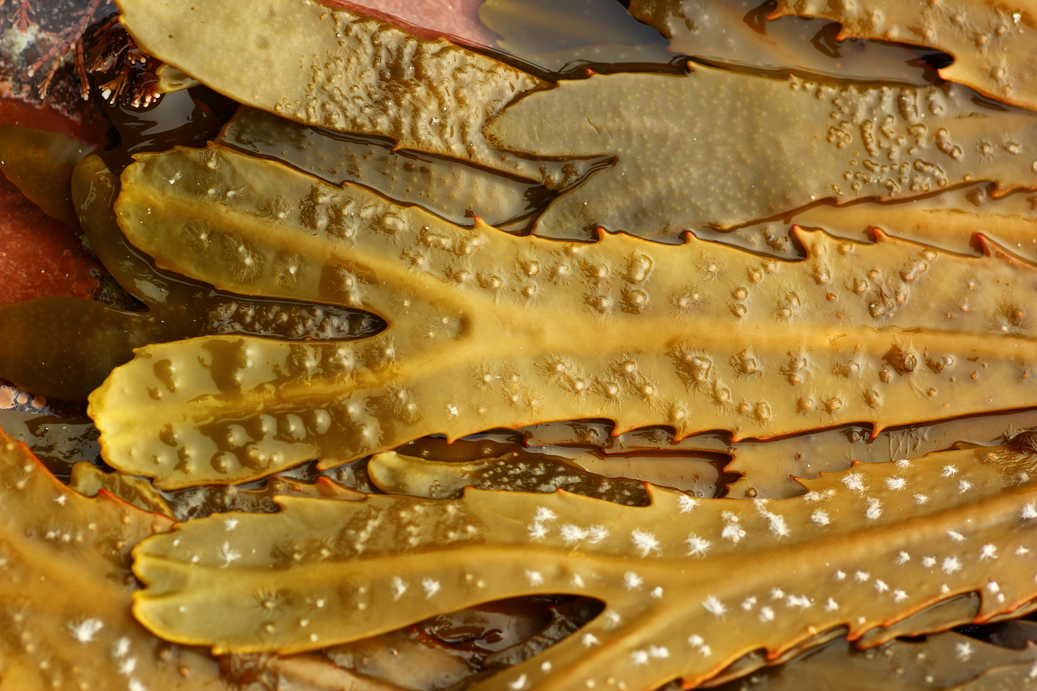
\includegraphics[width=3cm]{IMG_1667_r.png}};
\node [text width=3cm, text centered] at (8.4cm,-3.3cm) {\scriptsize{\textit{Fucus} \textit{serratus}}};

\end{tikzpicture}

\end{document}